\documentclass[12pt]{article}
\renewcommand{\contentsname}{Inhalt}
\usepackage{graphicx}
\usepackage[margin=25mm]{geometry}
\usepackage{multicol}
\usepackage[
backend=biber,
style=numeric,
sorting=nyt,
defernumbers=false
]{biblatex}
\usepackage{hyperref}
\hypersetup{
    colorlinks=true,
    linkcolor= black,
    filecolor=black,      
    urlcolor=black,
    pdftitle={NN Graph Classifier},
    pdfpagemode=FullScreen,
    citecolor=black,
    linktoc=all,
    pdfnewwindow=true,
    pageanchor=true,
    }

\graphicspath{ {./imgs/} }

\addbibresource{References.bib}

\title{NN Portfolio Optimierung}
\date{09. Februar 2024}
\author{Patrick Spohr}
\linespread{1.5} 

\begin{document}

    \begin{titlepage}
        
        \centering
        \Huge \textbf{Neural Network Graph Classifier}

        \vspace{7mm}
        
        \centering
        \Large \textit{of Probability Distributions} 

        \vspace{7mm}

        \centering
        \large by

        \vspace{7mm}

        \large Patrick Spohr
        \vspace{2mm}
        \\ 20th February 2024

        \vspace{30mm}

        \centering
        \large Master’s Program
        \vspace{1mm}
        \\ \normalsize \textit{Finanzmathematik, Aktuarwissenschaften und Risikomanagement} 

        \vspace{5mm}

        \centering
        \large Department
        \vspace{1mm}
        \\ \normalsize \textit{Informatik, Kommunikation und Wirtschaft} 

        \vspace{5mm}

        \centering
        \large Course 
        \vspace{1mm}       
        \\ \normalsize \textit{Statistical Learning in Finance and Insurance} 

        \vspace{5mm}

        \centering
        \large Professor
        \vspace{1mm}
        \\ \normalsize \textit{Dr. Alla Petukhina} 


    \end{titlepage}

    \hypertarget{Table of Contents}{\tableofcontents}

    \newpage

    \newpage \section{Motivation} 
    
        \subsection{Graph Classifier}
            
            
            

    \newpage \section{Objectives}

        \subsection{Main Goal}

           
        
        \subsection{Literature Overview}
        

        \subsection{Hurdles to Overcome}
        
    
        
    \newpage \section{Data}
            
        \subsection{CIFAR-10 Images}
    
           
            
        \subsection{Scraped Graphs}
    

            
          
            \begin{table}[htp]
                \begin{center}
                    
                    \begin{tabular}{ | l | l | l | l | l | }

                        \hline
                        \textbf{Ticker}      & \textbf{Name}                             & \textbf{Geschäft} \\
                        \hline
                        COHR                 & Coherent, Inc.                            & Laser \\
                        CTB                  & Cooper Tire \& Rubber Company             & Reifen \\
                        EQT                  & EQT Corporation                           & Energie \\
                        GOLD                 & Barrick Gold Corporation                  & Bergarbeit \\
                        NSEC                 & National Security Group, Inc.             & Versicherung \\
                        OTTR                 & Otter Tail Corporation                    & Energie \\
                        PEP                  & PepsiCo, Inc.                             & Getränke \\
                        SKYW                 & SkyWest, Inc.                             & Fluglinie \\
                        SNFCA                & Security National Financial Corporation   & Lebensversicherung \\
                        WY                   & Weyerhaeuser Company                      & Abholzung \\
                        \hline

                    \end{tabular}

                \end{center}
            \end{table}

        \subsection{Generated Graphs}
         

    \newpage \section{Methoden}

        \subsection{Overview}

           
            
            \begin{figure}[htp]
            
                \begin{center}

                    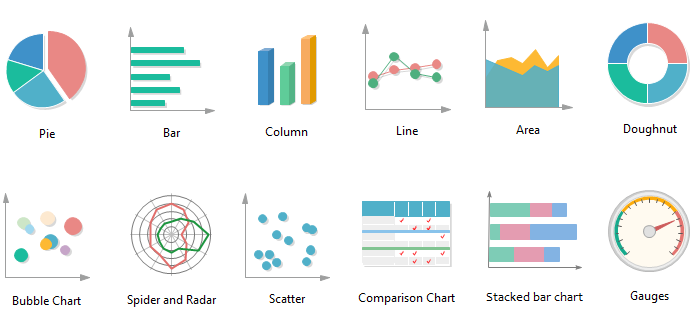
\includegraphics[scale=0.5]{types-of-graphs.png}
                    \caption{Feed-Forward Neuronales Netz \cite{bishop1995}}
        
                \end{center}
                
            \end{figure}
        
            

        \subsection{Feed-Forward Neural Networks}

          
            
            \begin{figure}[ht]
            
                \begin{center}

                    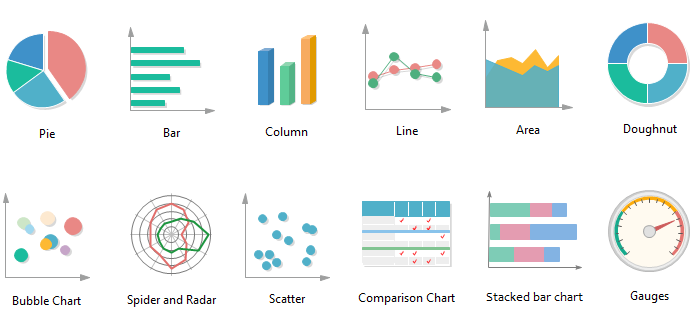
\includegraphics[scale=0.5]{types-of-graphs.png}
                    \caption{Long Short-Term Memory Unit \cite{yan2016}}
        
                \end{center}
                
            \end{figure}

          

        \subsection{Convolutional Neural Networks}

           

            \begin{figure}[ht]
            
                \begin{center}

                    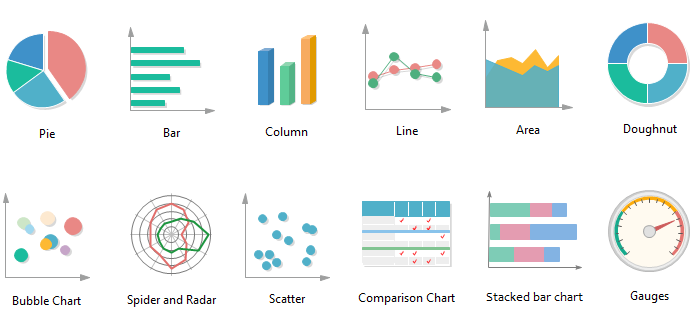
\includegraphics[scale=0.5]{types-of-graphs.png}
                    \caption{Long Short-Term Memory Unit \cite{data-basecamp}}
        
                \end{center}
                
            \end{figure}

        \subsection{Rectified Linear Units}

          

            \begin{multicols}{2}
                
                \begin{Large} \[ Sharpe = \frac{R_p - R_f}{\sigma_p} \] \end{Large}

                \vfill

                \begin{small}

                    \noindent $R_p$ = Portfolio Renditen \newline 
                    $R_f$ = risikofreier Zinssatz \newline 
                    $\sigma_p$ = Standardabweichung der Renditen 

                \end{small}

            \end{multicols}

         


        \subsection{Adam Optimizer}

          

            \begin{figure}[ht]
            
                \begin{center}

                    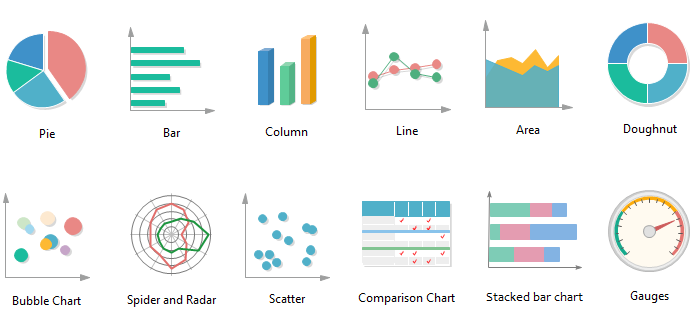
\includegraphics[scale=0.5]{types-of-graphs.png}
                    \caption{Long Short-Term Memory Unit \cite{zhang2020}}
        
                \end{center}
                
            \end{figure}


        \subsection{Python, Keras, and Libaries}
                
          
                
                
            \begin{table}[htp]

                \begin{center} 

                \scalebox{1.2}[1.2]{
                \begin{tabular}{ | c | c | }
                \hline
                \textbf{Library}    &       \textbf{Versionen} \\
                \hline
                python              &       3.10.13 \\ 
                tensorflow          &       2.10.0 \\
                numpy               &       1.26.0 \\
                pandas              &       2.1.1 \\
                matplotlib          &       3.8.0 \\
                
                \hline
                \end{tabular}
                }

                \caption{Python und Library Versionen}
                \label{pl-versionen}

                \end{center}

            \end{table}
       

        \subsection{Simplified Graph Classifier}

         

            \newpage
            \begin{Large} \[ V_p = \sum_{j=1}^{A}\sum_{i=1}^{M}P^T_{i+1} \cdot w_i \] \end{Large}

            \begin{multicols}{2}
                \begin{footnotesize}
                    
                    \noindent M = 360 Monate \\
                    A = 10 Aktien \\
                    P = tägliche Preise von Aktie A im Monat M \\
                    w = monatliche Gewicht von Aktie A im Monat M \\
                    $P_{1+1}$ = Preise im Februar 1990 von Aktie A \\
                    $w_1$ = Gewicht im Januar 1990 von Aktie A 

                \end{footnotesize}
            \end{multicols}

        \subsection{Distribution Graph Classifier}

    \section{Results}
    
        \subsection{Simple Graph Classifiers}

         


            \begin{figure}[ht]
            
                \begin{center}

                    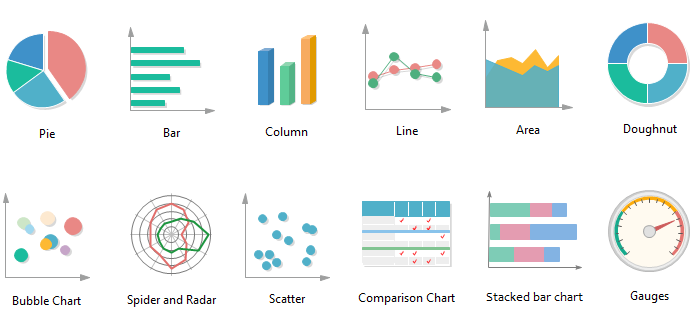
\includegraphics[scale=0.5]{types-of-graphs.png}
                    \caption{Normalisierte Portfoliowerte von 1990 bis 2020}
                    \label{n-portfoliowerte-fig}
        
                \end{center}
                
            \end{figure}

            
            

            \begin{figure}[ht]
            
                \begin{center}

                    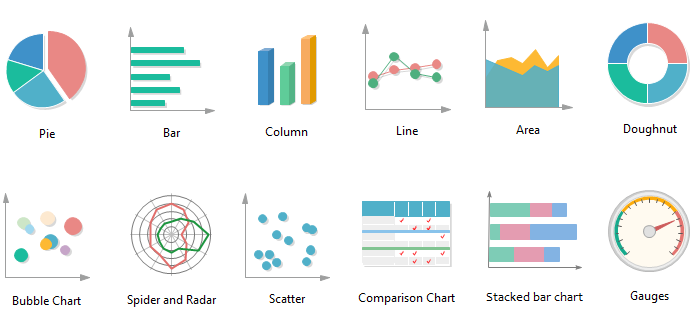
\includegraphics[scale=0.5]{types-of-graphs.png}
                    \caption{Summe monatlichen Renditen von 1990 bis 2020}
                    \label{s-m-renditen-fig}
        
                \end{center}
                
            \end{figure}


           

            \begin{table}[htp]
                \begin{center}
                    
                    \begin{tabular}{ | l | l | }

                        \hline
                        \textbf{Portfolio}   & \textbf{Summe Monatlichen Renditen \%} \\
                        \hline
                        OPT mit RFR          &      6604,73 \\            
                        OPT ohne RFR         &      5331,83 \\
                        EQU                  &      213,32 \\                 
                        GSPC                 &      248,56 \\          
                             
                        \hline

                    \end{tabular}
                    \caption{Summe Monatlichen Renditen}
                    \label{s-m-renditen-tab}
                \end{center}
            \end{table}

        \subsection{Distribution Graph Classifiers}

       

  
                
        \begin{table}[htp]
            \begin{center}
                
                \begin{tabular}{ | l | l | }

                    \hline
                    \textbf{Portfolio}   & \textbf{Monatlicher Durchschnitt} \\
                    \hline
                    OPT mit RFR          & 39,9735  \\          
                    OPT ohne RFR         & 41,1696 \\
                    EQU                  & 52,8962  \\              
                    GSPC                 & 72,302  \\       
                            
                    \hline

                \end{tabular}
                \caption{Gesamtsumme der Sharpe-Quotienten ohne den Risikofreinen Zinssatz}
                \label{gs-sq-ohne-rfz}

            \end{center}
        \end{table}

        \begin{table}[htp]
            \begin{center}
                
                \begin{tabular}{ | l | l | }

                    \hline
                    \textbf{Portfolio}   & \textbf{Monatlicher Durchschnitt} \\
                    \hline
                    OPT mit RFR          & -0,0026 \\      
                    OPT ohne RFR         & 0,0225 \\
                    EQU                  & 0,0934 \\            
                    GSPC                 & 1,7403 \\     
                            
                    \hline

                \end{tabular}
                \caption{Monatlicher Durchschnitt der Sharpe-Quotienten ohne den Risikofreinen Zinssatz}
                \label{md-sq-ohne-rfz}

            \end{center}
        \end{table}


        \begin{table}[htp]
            \begin{center}
                
                \begin{tabular}{ | l | l | }

                    \hline
                    \textbf{Portfolio}   & \textbf{Monatlicher Durchschnitt} \\
                    \hline
                    OPT mit RFR          & 30,2492  \\          
                    OPT ohne RFR         & 28,7633 \\
                    EQU                  & -345,5259  \\              
                    GSPC                 & -395,0716  \\       
                            
                    \hline

                \end{tabular}
                \caption{Gesamtsumme der Sharpe-Quotienten mit dem Risikofreinen Zinssatz}
                \label{gs-sq-mit-rfz}

            \end{center}
        \end{table}

        \begin{table}[htp]
            \begin{center}
                
                \begin{tabular}{ | l | l | }

                    \hline
                    \textbf{Portfolio}   & \textbf{Monatlicher Durchschnitt} \\
                    \hline
                    OPT mit RFR          & 0,08449 \\      
                    OPT ohne RFR         & 0,08034 \\
                    EQU                  & -0,9651 \\            
                    GSPC                 & -1,1035 \\     
                            
                    \hline

                \end{tabular}
                \caption{Monatlicher Durchschnitt der Sharpe-Quotienten mit dem Risikofreinen Zinssatz}
                \label{md-sq-mit-rfz}

            \end{center}
        \end{table}

        
        \newpage \subsection{Conclusions and Further Research}

       
    
    
    \printbibliography[heading=bibintoc, title={References}]


\end{document}